\documentclass{beamer}
\usetheme{metropolis}           % Use metropolis theme
\usepackage{graphicx} % For including images
\usepackage{url} % For handling URLs
\usepackage{tcolorbox} % For creating pretty boxes
\usepackage[numbers]{natbib} 
% \usepackage[style=alphabetic]{biblatex}

% Define a custom tcolorbox style for definitions
\tcbset{
    definitionstyle/.style={
        colback=blue!5!white, % Background color
        colframe=blue!75!black, % Border color
        fonttitle=\bfseries, % Bold title
        coltitle=white, % Title color
        boxrule=0.75mm, % Border thickness
        arc=2.5mm, % Rounded corners
        left=2mm, % Left padding
        right=2mm, % Right padding
        top=1mm, % Top padding
        bottom=1mm % Bottom padding
    }
}

% for the sources of images: very small footnotes
\newcommand{\sourcefootnote}[1]{\let\thefootnote\relax\footnote{{\tiny Source: \url{#1}}}}

\title{Temporal Graphs}

\date{\today}

\author{Daniel Cermann}

\institute{
  \hfill \begin{minipage}{0.3\textwidth}
    \begin{center}
      
\includegraphics[width=60px]{media/hpi_logo.png} \newline
      Hasso Plattner Institute 
    \end{center}
  \end{minipage}
}


\begin{document}

\begin{frame}
  \begin{center}
    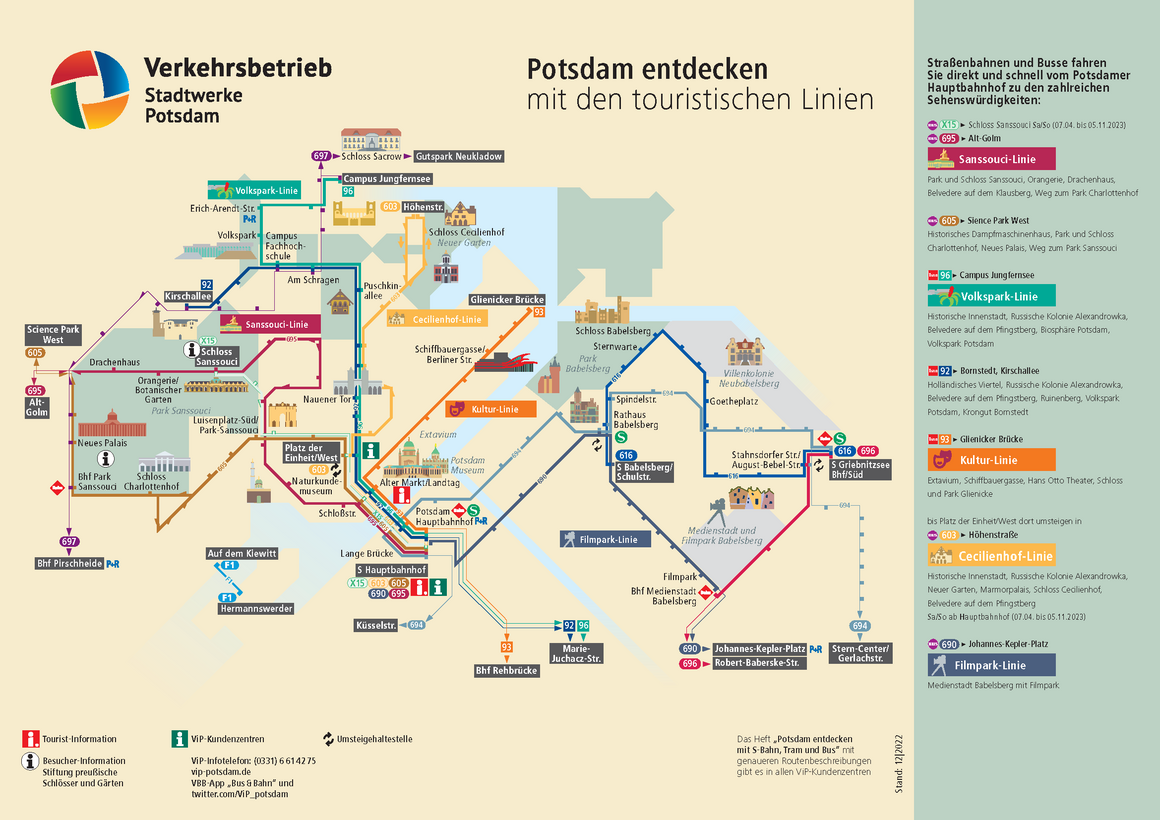
\includegraphics[width=0.95\textwidth]{media/potsdam_citynet.png}
  \end{center}
  \sourcefootnote{https://www.swp-potsdam.de/content/verkehr/bilder_6/liniennetz/touristischer_liniennetzplan_screenshot_1280_960.jpg}
\end{frame}

\maketitle

\section{Motivation}

\begin{frame}{Clip: School day}
  
\end{frame}

\begin{frame}{Google Maps}
  
\end{frame}

\begin{frame}{How to represent time in graphs?}

\end{frame}

\begin{frame}{Time matters!}
  - not transitive
\end{frame}
% insert some real-live applications here


\section{How to model temporal graphs}
\begin{frame}{Definition labeled graphs}
    \begin{tcolorbox}[definitionstyle, title=Definition]
      A \textbf{labeled graph} \citep[page 94]{GHOSH201888} is a triple \( G = (V, E, \lambda) \) where:
        \begin{itemize}
            \item \( V, E \) is a graph
            \item $ \lambda: V \cup E \rightarrow Z$ is a mapping of nodes and edges to a set of labels $Z$
          \end{itemize}
    \end{tcolorbox}
\end{frame}

\begin{frame}{Definition temporal graphs}
    \begin{tcolorbox}[definitionstyle, title=Definition]
      A \textbf{temporal graph} \citep[page 243]{Michail2015} is is triple \( G = (V, E, \lambda) \) where:
        \begin{itemize}
            \item \( V, E \) is a graph
            \item $ \lambda: E \rightarrow 2^{\mathbb{N}}$ is a mapping edges to a set natural numbers (time steps when this edge is active)
          \end{itemize}
    \end{tcolorbox}
\end{frame}

\begin{frame}{Notation for convenience $\rightarrow$ \citep[p. 243ff]{Michail2015}}
\begin{itemize}
  \item $\lambda(G)$ - temporal graph with respect to $G$
  \item $\lambda(E)$ - multiset of all labels
  \item $| \lambda | = \sum_{e \in E} | \lambda(e) | $
  \item $ \lambda_{min} = min\{l \in \lambda(E)\} $
  \item $ \lambda_{max} = max\{l \in \lambda(E)\} $
  \item $\alpha(\lambda) = \lambda_{max} - \lambda_{min} + 1$ - lifetime of a temporal graph $\lambda(G)$
\end{itemize}
\end{frame}

\begin{frame}{Notation #2}
\begin{itemize}
  \item A temporal graph $D$ is a an ordered set of disjoint sets $(V, A)$
  \item $A \subseteq V^2 \times \mathbb{N}$ - 'time edges'
  \item $A(t) = \{e | (e, t) \in A\}$ - set of edges at time $t$
  \item $D(t) = (V, A(t))$ - snapshot of graph D at time $t$
\end{itemize}
\end{frame}

\begin{frame}{Static expansion of a temporal graph}
  \begin{center}
    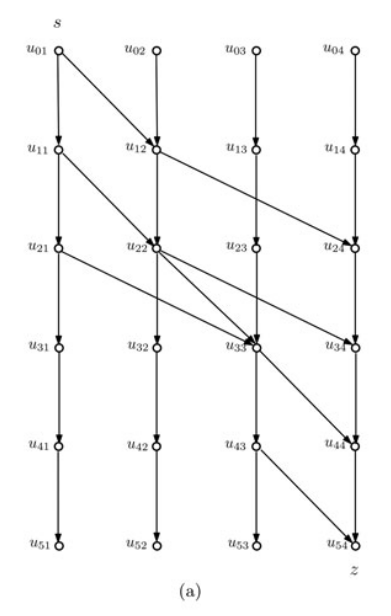
\includegraphics[height=0.8\textheight]{media/static_expansion_of_graphs.png}
  \end{center}
  \citep[page 318]{Michail2015}
\end{frame}

\begin{frame}{Static expansion of a temporal graph}
  \begin{tcolorbox}[definitionstyle, title=Definition: static expansion of a graph]
    The static expansion of a temporal graph $D = (V, A)$ with $V = \{ u_1, u_2, ..., u_n \}$ is a DAG $H = (S, E)$ with:
    $$ S = \{ u_{ij} | \lambda_{min} - 1 \leq i \leq \lambda_{max}, 1 \leq j \leq n \} $$
    and
    $$ E = \{ (u_{(i - 1)j}, u_{ij'}) | \lambda_{min} \leq i \leq \lambda_{max} \land $$
    $$ 1 \leq j, j' \leq n \land (j = j' \lor (u_j, u_{j'}) \in A(i))) \} $$
  \end{tcolorbox}
\end{frame}

\begin{frame}{Journeys}

\end{frame}


\section{Teasers}

\begin{frame}{Graph Neural Networks}

\end{frame}

\begin{frame}{Sources}
  \bibliographystyle{plain}
  \bibliography{references}
\end{frame}

\end{document}
